% $Header$
% MBDyn (C) is a multibody analysis code.
% http://www.mbdyn.org
%
% Copyright (C) 1996-2010
%
% Pierangelo Masarati  <masarati@aero.polimi.it>
%
% Dipartimento di Ingegneria Aerospaziale - Politecnico di Milano
% via La Masa, 34 - 20156 Milano, Italy
% http://www.aero.polimi.it
%
% Changing this copyright notice is forbidden.
%
% This program is free software; you can redistribute it and/or modify
% it under the terms of the GNU General Public License as published by
% the Free Software Foundation (version 2 of the License).
% 
%
% This program is distributed in the hope that it will be useful,
% but WITHOUT ANY WARRANTY; without even the implied warranty of
% MERCHANTABILITY or FITNESS FOR A PARTICULAR PURPOSE.  See the
% GNU General Public License for more details.
%
% You should have received a copy of the GNU General Public License
% along with this program; if not, write to the Free Software
% Foundation, Inc., 59 Temple Place, Suite 330, Boston, MA  02111-1307  USA

\section{Aerodynamic Elements}
\label{sec:EL:AERO}


\subsection{Aerodynamic Body/Aerodynamic Beam2/3}
\label{sec:EL:AERO:BODY-BEAM23}
These elements share the description of the aerodynamics.
The former assumes the aerodynamic surface to be rigid,
and takes its configuration from a single node, while the latter
respectively relie on a two or three-node beam
and use the same interpolation functions of the beam to compute
the configuration at an arbitrary point.

The input format is:
%\begin{verbatim}
\begin{Verbatim}[commandchars=\\\{\}]
    \bnt{elem_type} ::= \{ \kw{aerodynamic body} | \kw{aerodynamic beam2} | \kw{aerodynamic beam3} \}

    \bnt{normal_arglist} ::= \bnt{connectivity} ,
        (\ty{Shape<1D>})          \bnt{surface_chord} ,
        (\ty{Shape<1D>})          \bnt{surface_aerodynamic_center} ,
        (\ty{Shape<1D>})          \bnt{surface_b_c_point} ,
        (\ty{Shape<1D>})          \bnt{surface_twist} ,
        [ \kw{tip loss} , (\ty{Shape<1D>}) \bnt{tip_loss} , ]
        \bnt{integration_points}
        [ , \kw{control} , (\ty{DriveCaller}) \bnt{control_drive} ] 
        [ , \bnt{airfoil_data} ]
        [ , \kw{unsteady} , \{ \kw{bielawa} \} ]
        [ , \kw{jacobian} , \{ \kw{yes} | \kw{no} | \bnt{bool} \} ]
        [ , \bnt{custom_output} ]

    \bnt{extra_arglist} ::= \{ \kw{std} | \kw{gauss} | \kw{node} \}
\end{Verbatim}
%\end{verbatim}
where
%\begin{verbatim}
\begin{Verbatim}[commandchars=\\\{\}]
    \bnt{connectivity} ::= \{ \bnt{body_conn} | \bnt{beam2_conn} | \bnt{beam3_conn} \}

    # \bnt{elem_type} ::= \kw{aerodynamic body}
    \bnt{body_conn} ::= \bnt{node_label}
        [ , [ \kw{user defined} ] \kw{induced velocity} , \bnt{induced_velocity_label} ] ,
        (\ty{Vec3})              <relative_surface_offset> , 
        (\ty{OrientationMatrix}) <relative_surface_orientation> ,
        (\ty{Scalar})            <surface_span>

    # \bnt{elem_type} ::= \kw{aerodynamic beam2}
    \bnt{beam2_conn} ::= \bnt{beam2_label}
        [ , [ \kw{user defined} ] \kw{induced velocity} , \bnt{induced_velocity_label} ] ,
        (\ty{Vec3})              \bnt{relative_surface_offset_1} ,
        (\ty{OrientationMatrix}) \bnt{relative_surface_orientation_1} ,
        (\ty{Vec3})              \bnt{relative_surface_offset_2} ,
        (\ty{OrientationMatrix}) \bnt{relative_surface_orientation_2} ,

    # \bnt{elem_type} ::= \kw{aerodynamic beam3}
    \bnt{beam3_conn} ::= \bnt{beam3_label} 
        [ , [ \kw{user defined} ] \kw{induced velocity} , \bnt{induced_velocity_label} ] ,
        (\ty{Vec3})              \bnt{relative_surface_offset_1} ,
        (\ty{OrientationMatrix}) \bnt{relative_surface_orientation_1} ,
        (\ty{Vec3})              \bnt{relative_surface_offset_2} ,
        (\ty{OrientationMatrix}) \bnt{relative_surface_orientation_2} ,
        (\ty{Vec3})              \bnt{relative_surface_offset_3} ,       
        (\ty{OrientationMatrix}) \bnt{relative_surface_orientation_3} ,

    \bnt{airfoil_data} ::=
        \{ \kw{naca 0012}
            | \kw{rae 9671}
            | [ \kw{theodorsen} , ] \kw{c81} , \bnt{c81_data} \}
\end{Verbatim}
%\end{verbatim}
and
%\begin{verbatim}
\begin{Verbatim}[commandchars=\\\{\}]
    \bnt{c81_data} ::=
        \{ \bnt{c81_label}
            | \kw{multiple} , \bnt{airfoil_number} ,
                \bnt{c81_label} , \bnt{end_point}
                [ , ... ]
            | \kw{interpolated} , \bnt{airfoil_number} ,
                \bnt{c81_label} , \bnt{position}
                [ , ... ] \}
\end{Verbatim}
%\end{verbatim}
The \nt{custom\_output} optional data consists in
%\begin{verbatim}
\begin{Verbatim}[commandchars=\\\{\}]
    \bnt{custom_output} ::= \kw{custom output} , 
        \bnt{custom_output_flag} [ , ... ]
\end{Verbatim}
%\end{verbatim}
The values of \nt{custom\_output\_flag}
are defined in Section~\ref{sec:CONTROLDATA:DEFAULTAERODYNAMICOUTPUT}.

Flags add up to form the custom output request.
Flags may not be repeated.
By default, only forces are output.
The custom output is only available in NetCDF format;
see Section~\ref{sec:NetCDF:Elem:Aerodynamic}.

The field \nt{induced\_velocity} indicates the label
of the \kw{induced velocity} element that this element is linked to.
This means that the element can get information about the
induced velocity and should supply information about the forces it generates.
If the keyword \kw{user defined induced velocity} is used,
then \nt{induced\_velocity} refers to a \kw{user defined} element.
Note: if the keyword \kw{induced velocity} is used
and no induced velocity element is found with the label \nt{induced velocity}
a \kw{user defined} element with that label is looked up.

An arbitrary relative orientation and offset is allowed for all elements with
respect to the nodes they are linked to. 
This means that the aerodynamic beam offsets refer to the position
of the beam's nodes, and have nothing to do with offsets related
to the structural beam element.

The \ty{Shape<1D>} entities are used to compute the physical chord,
aerodynamic center, velocity measurement point (the point where the
kinematic boundary conditions are evaluated) and twist as functions 
of the dimensionless abscissa along the span.

The optional \kw{tip loss} keyword allows to define an additional shape,
\nt{tip\_loss},
whose value is used to scale the value of the normal aerodynamic force.
By default, the scale factor is 1.
The \nt{tip\_loss} shape should have a value comprised between 0 and 1.

In any case, the user must be aware of the fact that Gauss integration
will be used over the span of the element.
This consists in evaluating forces at specific spanwise stations.
This assumes that the function to be integrated over the spanwise domain
is regular.
Sharp variations, like tip loss concentrated in the outmost 2\%
of a rotor blade span, might be entirely missed when using too little
spanwise elements with too little integration points.

The span of the \kw{aerodynamic body} element is set by the user;
the offset vector points to the center-span of the element.
The span of the \kw{aerodynamic beam2} and \kw{aerodynamic beam3} elements
is computed based on the metric of the beam, from the first to the last node.

The aerodynamic center and the velocity measurement points are measured
relative to the centerline of the elements, that is the line in direction 3
of the local frame from the end of the offset vector.
This line is assumed to be at the 25\% of the airfoil chord when steady
aerodynamic coefficients are used (\nt{unsteady\_flag} = 0).
The direction 1 is assumed to be the ``reference'' line of the airfoil, 
from the trailing edge to the leading edge (points ``forward''),
while direction 2 is normal to the other two and goes from the lower 
to the upper side of the airfoil (points ``up''). 
Figure~\ref{fig:AIRFOIL} shows the arrangement of the airfoil geometry 
and properties.

\begin{figure}[h]
  \centering
    %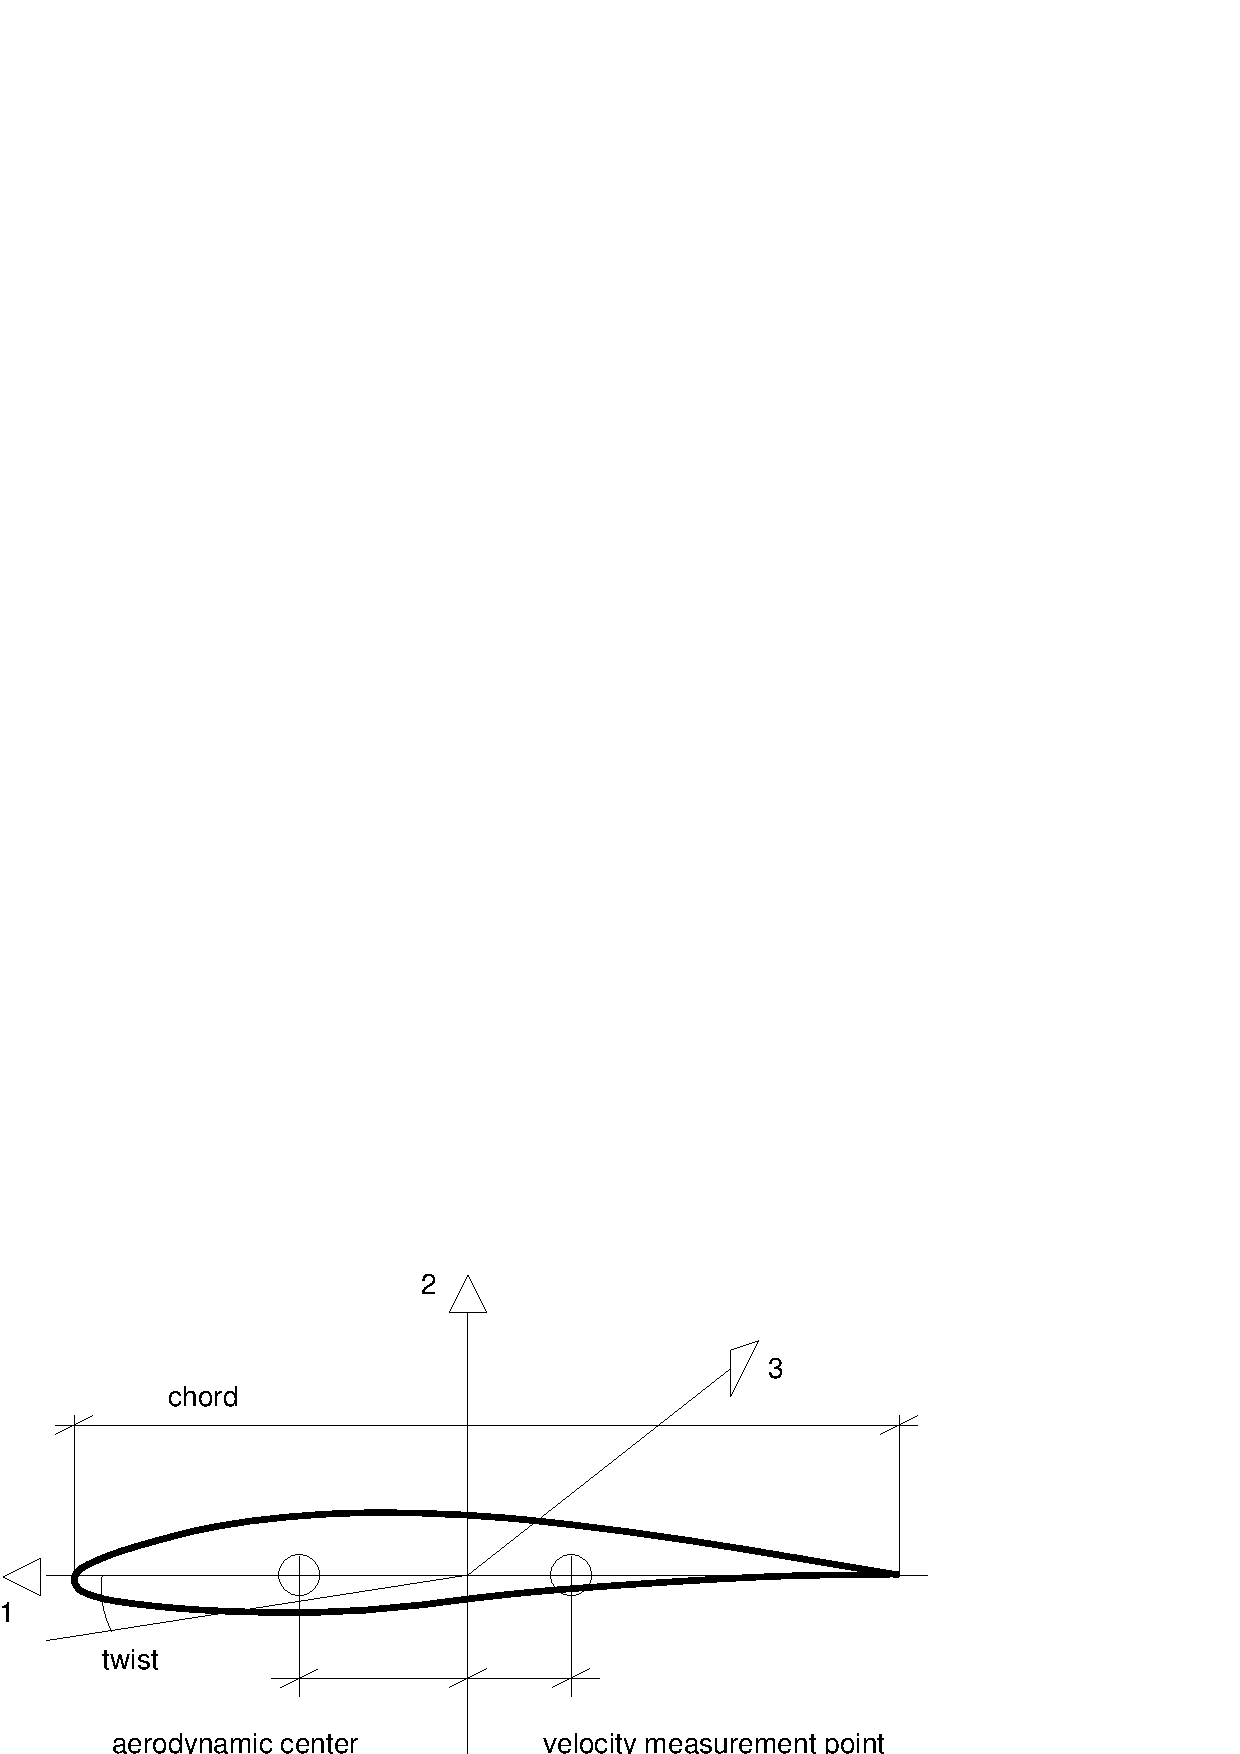
\includegraphics[width=80mm]{airfoil.pdf}
    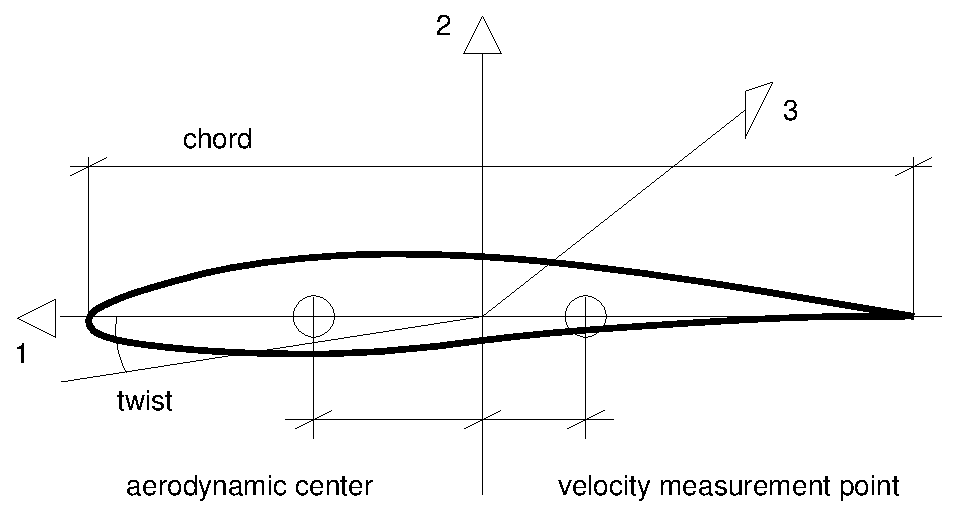
\includegraphics[width=80mm]{airfoil.eps}
  \caption{Airfoil geometry}\label{fig:AIRFOIL}
\end{figure}

The \nt{airfoil\_data} defaults to a built-in NACA 0012 semi-analytical
model (FIXME: the unsteady correction is buggy; use the \kw{c81} 
mode instead).

The \kw{multiple} mode of the c81 data allows to specify
more than one airfoil for an aerodynamic element; the transition
between airfoils is sharp.
The integer \nt{airfoil\_number} indicates how many airfoils are expected;
the real \nt{end\_point} indicates where the influence zone for that
airfoil ends, expressed in terms of a non-dimensional abscissa spanning 
$\plbr{-1,1}$ along the reference line, roughly along axis 3 
of the aerodynamic reference frame; \nt{end\_point} must not lie outside
the element.
So, for example, if airfoil NACA 0015 is used in the leftmost part
of an element up to 1/4 span, NACA 0012 is used from 1/4 to 3/4 span,
and NACA 0009 is used in the remaining rightmost 1/4, the syntax is:
\begin{verbatim}
    set: integer naca0015 = 15;
    set: integer naca0012 = 12;
    set: integer naca0009 = 9;
    c81 data: naca0015, "naca0015.c81";
    c81 data: naca0012, "naca0012.c81";
    c81 data: naca0009, "naca0009.c81";
    # beginning of aerodynamic element definition...
        multiple, 3,
            naca0015, -0.5,    # from -1.0 to -0.5
            naca0012,  0.5,    # from -0.5 to  0.5
            naca0009,  1.0,    # from  0.5 to  1.0
    # ...rest of aerodynamic element definition
\end{verbatim}

The \kw{interpolated} mode of the \kw{c81} data allows to specify 
a smooth transition between different airfoils inside an element.
The interpolation occurs at the integration points where the
aerodynamic data is required, and it is performed once for all
at the beginning of the analysis.
Since this operation is time consuming, and essentially unnecessary,
the interpolated data can be generated once for all with the utility
\texttt{util/c81merge} once the position of the integration point is known,
and the \kw{multiple} mode can be used to directly provide
the interpolated data to the aerodynamic element.

The \kw{theodorsen} aerodynamic data uses C81 data,
and superimposes Wagner's approximation of the Theodorsen incompressible
unsteady correction of 2D lift and moment coefficients.
It is experimental.

The \nt{extra\_arglist} allows to define the style of the output.
The \kw{std} style (the default), the \kw{gauss} and the \kw{node}
styles are illustrated in the output section.


\subsubsection{Output}
Aerodynamic elements, both bodies and beams, write their output with file
extension \texttt{.aer}; for each time step the required elements are output.
In any case the label of the element is output first.
Three different formats are available: \kw{std} (the default),
\kw{gauss} and \kw{node}.

\begin{itemize}
\item[\kw{std}] (or Coefficients at Gauss points):
the output consists in a set of 8 numbers
for each block, that describe data at each Gauss integration point;
multiple blocks for a single element are written on the same line.
The format is:
\begin{itemize}
    \item the angle of attack at that station, in degrees 
	(namely, the angle between the component of the airfoil velocity,
	evaluated at the velocity measurement point, that in the airfoil
	plane and a reference line on the airfoil)
    \item the local yaw angle, in degrees
	(namely, the angle whose tangent is the ratio
	between the axial and the inplane components of the airfoil
	velocity)
    \item the local Mach number
    \item the local lift coefficient
    \item the local drag coefficient
    \item the local aerodynamic moment coefficient
    \item a private number
    \item another private number
\end{itemize}
When \kw{aerodynamic beam2} and \kw{aerodynamic beam3} elements are considered,
the output is repeated for each portion of the beam; so, for example,
a two-node beam is split in two portions, so the output
contains $2\times \nt{integration\_points}$ data blocks,
while a three-node beam is split in three portions,
so the output contains $3\times \nt{integration\_points}$ data blocks.

\item[\kw{node}:]
the format is:
\begin{itemize}
    \item the label of the node
    \item the three components of the force applied to the node
    \item the three components of the couple applied to the node
\end{itemize}
When \kw{aerodynamic beam2} and \kw{aerodynamic beam3} elements are considered,
the output is repeated on the same line for each node
the element is connected to.

\item[\kw{gauss}] (or Forces at Gauss points):
the output consists in the forces and moments
per unit length at each Gauss integration point; the format is:
\begin{itemize}
    \item the direction of the wind velocity relative to the element frame
    \item the lift,
    \item the drag,
    \item and the aerodynamic moment per unit length
\end{itemize}
When \kw{aerodynamic beam2} \and \kw{aerodynamic beam3} elements are considered,
the output is repeated on the same line for each portion of beam.
\end{itemize}



\subsection{Aeromodal Element}
\emph{Note: prepared by Alessandro Scotti.}

\noindent
This element is used to model an aerodynamic modal element,
i.e.\ an unsteady aerodynamic model that inherits the structural 
motion from a  \htmlref{\kw{modal}}{sec:EL:STRUCT:JOINT:MODAL} element
Its definition is very similar to that of the pure modal element, 
but it also includes some data representing unsteady aerodynamics 
in the time domain trough the residualization matrices.
This element is defined as follows:
%\begin{verbatim}
\begin{Verbatim}[commandchars=\\\{\}]
    \bnt{elem_type} ::= \kw{aeromodal}

    \bnt{normal_arglist} ::= 
        \bnt{reference_modal_joint} ,
        (\ty{OrientationMatrix}) \bnt{orientation} ,
        \bnt{reference_chord} ,
        \bnt{number_of_aerodynamic_states} ,
        [ \kw{rigid} , ]
        " \bnt{modal_matrices_file} "
\end{Verbatim}
%\end{verbatim}
With this formulation, anytime an aeromodal element is defined, 
the user needs to declare the number of modal aerodynamic elements 
in use in the \kw{control data} section.
An \htmlref{\kw{air properties}}{sec:EL:AERO:AIRPROPERTIES}
card definition is also required.

The keyword \kw{rigid} indicates that the generalized aerodynamic forces
provided by the model include global forces and moments associated 
to the rigid body motion of the underlying modal element (FIXME: untested).

There is also an optional gust model which is totally undocumented;
for further information, please contact the Author(s).

The \nt{modal\_matrices\_file} file includes the state space model in form 
of matrices $\T{A}$, $\T{B}$, $\T{C}$, $\T{D}_0$, $\T{D}_1$ and $\T{D}_2$,
according to the representation
\begin{align*}
	\dot{\T{x}} &= \T{A}\T{x} + \T{B}\T{q} \\	
	\T{f} &= q\plbr{\T{C}\T{x} + \T{D}_0 \T{q} + \frac{2V_{\infty}}{c} \T{D}_1 \dot{\T{q}} + \plbr{\frac{2V_{\infty}}{c}}^2 \T{D}_2 \ddot{\T{q}}}
\end{align*}
where $\T{q}$ are the modal variables that describe the structural motion,
and $\T{f}$ are the unsteady aerodynamic forces that apply to the structural
dynamics equations.

The file is formatted as follows:
\begin{verbatim}
    *** MATRIX A
    (<na> x <na> coefficients)
    *** MATRIX B
    (<na> x <ns> coefficients)
    *** MATRIX C
    (<ns> x <na> coefficients)
    *** MATRIX D0
    (<ns> x <ns> coefficients)
    *** MATRIX D1
    (<ns> x <ns> coefficients)
    *** MATRIX D2
    (<ns> x <ns> coefficients)
\end{verbatim}

\paragraph{Example.} \
\begin{verbatim}
    aeromodal: WING, WING_JOINT,
        eye,
        131.25, 10, "ha145b.fea";
\end{verbatim}
The \kw{aeromodal} element is declared with the label \texttt{WING}.
This element is attached to a \kw{modal} joint 
named \texttt{WING\_JOINT}.
The orientation of the aerodynamic reference with respect 
to the nodal reference is here expressed by the identity matrix (\kw{eye}).
The aerodynamic element chord is 131.25 inches.
This quantity must be consistent with the system chosen to define 
the whole model (SI, for example; in this case, British Units).
The next field, 10, indicates the number of states needed to use 
the aerodynamic model.
\texttt{ha145b.fea} is the name of the file that contains
the state space model matrices, obtained with an approximation 
chosen by the user.
In this particular case, a 10 states Pad\'e approximation 
has been chosen.
This example is taken from the Bisplinghoff Ashley Halfman
(BAH) Jet Transport Wing cantilevered wing with modal aerodynamic 
frequency responce, computed by a double-lattice method at Mach 0.0.
Data were extracted from the MSC-NASTRAN aeroelastic example file, 
named \texttt{ha145b}, while the aerodynamic state-space fitting 
has been computed using a Pad\'e polynomial approximation
(by Pasinetti \& Mantegazza).
All quantities are expressed in inches and pounds.



\subsection{Aircraft Instruments}
%\begin{verbatim}
\begin{Verbatim}[commandchars=\\\{\}]
    \bnt{elem_type} ::= \kw{aircraft instruments}

    \bnt{normal_arglist} ::= \bnt{aircraft_node}
        [ , \kw{orientation} , (\ty{OrientationMatrix}) \bnt{relative_orientation} ]
\end{Verbatim}
%\end{verbatim}
The \nt{aircraft\_node} represents the aircraft; it is assumed
that the ``nose'' of the aircraft is toward the positive $x$ direction
of the node, and the ``top'' of the aircraft is toward the positive 
$z$ direction of the node.
An optional orientation can be added to change the orientation 
of the aircraft with respect to the node.
This is useful, for example, with helicopters, where conventionally
the positive direction of the $x$ axis is nose to tail.

The available measures are accessed during the simulation 
by defining appropriate \kw{parameter} nodes, and by binding
the \kw{aircraft instruments} element private data to the nodes 
by means of the \kw{bind} mechanism, or directly by means
of the 
\hyperref{\kw{element} drive}{\kw{element} drive (see Section~}{)}{sec:DRIVE:ELEMENT}.

\paragraph{Private Data}
The following data is available:
\begin{itemize}
\item \kw{"airspeed"} the airspeed as seen by the reference 
	point on the aircraft, i.e. the combination 
	of the airstream speed and of the node speed
\item \kw{"groundspeed"} the absolute value of the projection
	of the node speed in the $xy$ plane.
\item \kw{"altitude"} the $z$ component of the node position
\item \kw{"attitude"} $\tan^{-1}\plbr{r_{31}, r_{11}}$
	(FIXME: better $\arcsin\plbr{r_{31}}$?)
\item \kw{"bank"} $\tan^{-1}\plbr{r_{32}, r_{22}}$
	(FIXME: better $\arcsin\plbr{r_{32}}$?)
\item \kw{"turn"} (not available yet)
\item \kw{"slip"} (not available yet)
\item \kw{"verticalspeed"} the $z$ component of the node velocity
\item \kw{"angleofattack"} the angle between the $z$ 
\item \kw{"heading"} the angle between the $x$ axis of the aircraft 
	and the ``north'' (the global $x$ axis) about the global $z$ axis;
	note: heading wraps about South
	(+180 deg from East, -180 deg from West).
\item \kw{"longitude"} (FIXME: not implemented yet)
\item \kw{"latitude"} (FIXME: not implemented yet)
\end{itemize}

\noindent
\emph{Note: this element is eXperimental.}




\subsection{Air Properties}\label{sec:EL:AERO:AIRPROPERTIES}
The properties of the airstream are made of the physical properties
of the air plus the description of the airstream velocity direction
and amplitude.
The former can be expressed in different forms, while the latter
are based on three-dimensional drive callers, \ty{TplDriveCaller<Vec3>}.
%\begin{verbatim}
\begin{Verbatim}[commandchars=\\\{\}]
    \bnt{arglist} ::=
        \{ (\ty{DriveCaller}) \bnt{air_density} , (\ty{Scalar}) \bnt{sound_celerity}
            | \kw{std} , \{ \{ \kw{SI} | \kw{British} \}
                [ , \kw{temperature deviation} , \bnt{delta_T} ]
                | \bnt{p0} , (\ty{DriveCaller}) \bnt{rho0} ,
                    \bnt{T0} , \bnt{dT/dz} , \bnt{R} , \bnt{g0} , \bnt{z1} , \bnt{z2} \}
            [ , \kw{reference altitude} , \bnt{z0} ] \} ,
        (\ty{TplDriveCaller<Vec3>}) \bnt{air_speed}
        [ , \kw{gust} , \bnt{gust_model} [ , ... ] ]
\end{Verbatim}
%\end{verbatim}
The first form consists in the bare input of the air density,
in form of a drive caller, and of the sound celerity, e.g.:
\begin{verbatim}
    air properties: 1.225, 340.,
        1.,0.,0., 150.;
\end{verbatim}
The second form uses standard air properties, both in the
international system (SI) or in British units, possibly
with a temperature deviation and an altitude offset, e.g.:
\begin{verbatim}
    air properties: std, SI, temperature deviation, -55,
        reference altitude, 1000.,
        1.,0.,0., 150.;
\end{verbatim}
where standard properties in SI are used, with a temperature
deviation of -55 K and a reference altitude of 1000 m.
The air properties are computed based on the $z$ position of the
point where the \kw{air properties} are requested (plus the optional
altitude offset).
The last possibility lets the user input all the parameters
required to compute the \kw{air properties} based on the $z$ position
of the point where they are requested, namely the reference
pressure \nt{p0}, the reference density \nt{rho0},
the reference temperature \nt{T0}, the initial temperature
gradient \nt{dT/dz}, the gas constant \nt{R}, the
initial gravity acceleration \nt{g0}, the bottom and top
altitudes of the null temperature gradient region \nt{z1} and
\nt{z2}; e.g., for SI units:
\begin{verbatim}
    air properties: std,
        101325.,       /* Pa */
        1.2250,        /* kg/m^3 */
        288.16,        /* K */
        -6.5e-3,       /* K/m */
        287.,          /* J/kgK */
        9.81,          /* m/s^2 */
        11000.,        /* m */
        25000.,        /* m */
        temperature deviation, -55,
        reference altitude, 1000.,
        1.,0.,0., 150.;
\end{verbatim}
The asymptotic air properties are characterized by the \ty{TplDriveCaller<Vec3>}
of the air speed, in the global reference frame.

\subsubsection{Gust}
If the optional \kw{gust} keyword is used, a gust model can be added.
Note that a very elementary gust model, represented by a uniform change
in airstream speed and direction can be implemented by using
a time-dependent airstream drive.

Gusts can also be appended later to the \kw{air properties} element
by using the statement
%\begin{verbatim}
\begin{Verbatim}[commandchars=\\\{\}]
    \kw{gust} : \bnt{gust_model} ;
\end{Verbatim}
%\end{verbatim}


\paragraph{Front 1D Gust}
The syntax of the \kw{front 1D} gust model is:
%\begin{verbatim}
\begin{Verbatim}[commandchars=\\\{\}]
    \bnt{gust_model} ::= \kw{front 1D} ,
        (\ty{Vec3})        \bnt{front_direction} ,
        (\ty{Vec3})        \bnt{perturbation_direction} ,
        (\ty{Scalar})      \bnt{front_velocity} ,
        (\ty{DriveCaller}) \bnt{front_profile}
\end{Verbatim}
%\end{verbatim}
This model consists in a uniform front, defined as
\begin{displaymath}
	\T{v}\plbr{\T{x}, t} = \T{n} g\plbr{\T{f} \cdot \T{x} + V_{ref} \cdot t}
\end{displaymath}
where
\begin{itemize}
\item $\T{v}$ is the velocity perturbation;
\item $\T{x}$ is the position of the point whose airstream velocity
is being computed;
\item $t$ is the current time;
\item $\T{n}$ is the unit vector \nt{perturbation\_direction} 
that defines the direction of the velocity perturbation;
\item $g\plbr{\cdot}$ is the function \nt{front\_profile} 
that defines the gust profile;
\item $\T{f}$ is the unit vector \nt{front\_direction} 
that defines the direction of propagation of the front;
\item $V_{ref}$ is the velocity \nt{front\_velocity} 
of propagation of the front in direction $\T{f}$.
\end{itemize}
As an example, a transverse cosine-shaped gust, with a wavelength of 100 m
and a peak velocity of 5 m/s moving downstream at the airstream speed,
100 m/s, in standard air, is presented:
\begin{verbatim}
    set: real waveLength = 100.; # m
    set: real V_inf = 100.;      # m/s
    set: real V_g = 5.;          # m/s
    air properties: std, SI,
        1.,0.,0., const, V_inf,  # reference airstream along X
        gust, front 1D,
            1.,0.,0.,            # front moving along X
            0.,0.,1.,            # gust along Z
            V_inf,               # front moving at V_inf
            cosine, 0., pi/waveLength, V_g/2., one, 0.;
\end{verbatim}



\paragraph{Scalar Function Wind Profile}
The syntax of the \kw{scalar function} wind profile,
implemented as a gust model within the \kw{air properties}, is:
%\begin{verbatim}
\begin{Verbatim}[commandchars=\\\{\}]
    \bnt{gust_model} ::= \kw{scalar function} ,
        \kw{reference position} , (\ty{Vec3}) \bnt{X0} ,
        \kw{reference orientation} , (\ty{OrientationMatrix}) \bnt{R0} ,
        (\ty{ScalarFunction}) \bnt{sf}
\end{Verbatim}
%\end{verbatim}
It yields a uniform velocity profile along the $x$ axis of the
reference orientation as a function of the $z$ axis component
of the relative position; namely, given the relative position
\begin{align}
	z &= \T{e}_3 \cdot \plbr{\T{x} - \nt{X0}}
	,
\end{align}
the velocity is
\begin{align}
	\T{v}
	&=
	\T{e}_1 \cdot \nt{sf}(z)
	,
\end{align}
where $\T{e}_i$ is the $i$-th axis of the reference orientation \nt{R0}.



\paragraph{Power Law Wind Profile}
The syntax of the \kw{power law} wind profile, implemented as a gust model
within the \kw{air properties}, is:
%\begin{verbatim}
\begin{Verbatim}[commandchars=\\\{\}]
    \bnt{gust_model} ::= \kw{power law} ,
        \kw{reference position} , (\ty{Vec3}) \bnt{X0} ,
        \kw{reference orientation} , (\ty{OrientationMatrix}) \bnt{R0} ,
        \kw{reference elevation} , \bnt{z_ref} ,
        \kw{reference velocity} , (\ty{DriveCaller}) \bnt{v_ref} ,
        \kw{exponent} , \bnt{exponent}
\end{Verbatim}
%\end{verbatim}
It yields a uniform velocity profile along the $x$ axis of the
reference orientation as a function of the $z$ axis component
of the relative position; namely, given the relative position
\begin{align}
	z &= \T{e}_3 \cdot \plbr{\T{x} - \nt{X0}}
	,
\end{align}
the velocity is
\begin{align}
	\T{v}
	&=
	\T{e}_1 \cdot \nt{v\_ref} \plbr{\frac{z}{\nt{z\_ref}}}^{\nt{exponent}}
	,
\end{align}
where $\T{e}_i$ is the $i$-th axis of the reference orientation \nt{R0}.
Typical values of \nt{exponent} are about 0.1.



\paragraph{Logarithmic Wind Profile}
The syntax of the \kw{logarithmic} wind profile, implemented as a gust model
within the \kw{air properties}, is:
%\begin{verbatim}
\begin{Verbatim}[commandchars=\\\{\}]
    \bnt{gust_model} ::= \kw{logarithmic} ,
        \kw{reference position} , (\ty{Vec3}) \bnt{X0} ,
        \kw{reference orientation} , (\ty{OrientationMatrix}) \bnt{R0} ,
        \kw{reference elevation} , \bnt{z_ref} ,
        \kw{reference velocity} , (\ty{DriveCaller}) \bnt{v_ref} ,
        \kw{surface roughness length} , \bnt{z_0}
\end{Verbatim}
%\end{verbatim}
It yields a uniform velocity profile along the $x$ axis of the
reference orientation as a function of the $z$ axis component
of the relative position; namely, given the relative position
\begin{align}
	z &= \T{e}_3 \cdot \plbr{\T{x} - \nt{X0}}
	,
\end{align}
the velocity is
\begin{align}
	\T{v}
	&=
	\T{e}_1 \cdot \nt{v\_ref} \cdot \frac{
		\log(z/\nt{z\_0}) - \psi_m
	}{
		\log(\nt{z\_ref}/\nt{z\_0}) - \psi_m
	}
	,
\end{align}
where $\T{e}_i$ is the $i$-th axis of the reference orientation \nt{R0}.

The surface roughness length describes the typical roughness
of the surrounding surface.
It is a very small number in case of smooth surface
(e.g.\ 0.01m for grass),
or 1/20 to 1/30 of the typical obstacle's size (e.g.\ 1m for woods).


\paragraph{Output}
The output occurs in the \texttt{.air} file, which contains:
\begin{itemize}
\item a fake label, always set to 1
\item the air density
\item the sound celerity
\item the three components of the reference air speed
with respect to the inertial reference frame
\end{itemize}


\paragraph{Private Data}
The following data is available:
\begin{itemize}
\item \kw{"vxinf"} the $x$ component of the airstream speed (without any gust contribution)
\item \kw{"vyinf"} the $y$ component of the airstream speed (without any gust contribution)
\item \kw{"vzinf"} the $z$ component of the airstream speed (without any gust contribution)
\item \kw{"vinf"} the module of the airstream speed (without any gust contribution)
\end{itemize}



\subsection{Generic Aerodynamic Force}
\label{sec:EL:AERO:GAF}
This element is experimental.
%\begin{verbatim}
\begin{Verbatim}[commandchars=\\\{\}]
    \bnt{elem_type} ::= \kw{generic aerodynamic force}

    \bnt{normal_arglist} ::= \bnt{node_label} ,
        [ \kw{position} , \bnt{relative_position} , ]
        [ \kw{orientation} , \bnt{relative_orientation} , ]
        [ \kw{reference surface} , \bnt{reference_surface} , ]
        [ \kw{reference length} , \bnt{reference_length} , ]
        \{ \bnt{data_file_specification} | \kw{reference} , \bnt{gaf_data_label} \}

    \bnt{data_file_specification} ::= \kw{file} , 
        [ \{ \kw{angle units} , \{ \kw{radians} | \kw{degrees} \}
            | \kw{scale angles} , \bnt{angle_scale_factor} \} , ]
        [ \kw{scale lengths} , \bnt{length_scale_factor} , ]
        " \bnt{data_file_name} "
\end{Verbatim}
%\end{verbatim}

\paragraph{Output}
The following output is available:
\begin{enumerate}
\item column 1: element label
\item column 2: the angle of attack $\alpha$
\item column 3: the sideslip angle $\beta$
\item columns 4--6: force components in local $x$, $y$ and $z$ directions
\item columns 7--9: moment components in local $x$, $y$ and $z$ directions,
	about the reference point (node plus offset)
\item columns 10--12: force components in global $x$, $y$ and $z$ directions
\item columns 13--15: moment components in global $x$, $y$ and $z$ directions,
	about the node
\end{enumerate}

\paragraph{Private Data}
The \kw{generic aerodynamic force} element does not output any private data.

\subsubsection{Generic Aerodynamic Element Data}
Data is stored in ASCII format in a file.

An arbitrary number of comment lines is allowed at the beginning.
Comment lines start with either a percent `\textbf{\%}'
or a hash mark `\texttt{\#}' in the first column.
Their content is discarded until the end of the line.

The first non-comment line must contain two integers separated by whitespace.
The integers represent the expected number of angle of attack
and sideslip angle values, $N_\alpha$ and $N_\beta$.

Another arbitrary number of comment lines is allowed.

A set of $N_\alpha \cdot N_\beta$ lines is expected.
No comments or empty lines are allowed in between.
Each line contains:
\begin{itemize}
\item column 1: the angle of attack, $\alpha$
\item column 2: the sideslip angle, $\beta$
\item columns 3--5: the force coefficients $f_{x/q}$, $f_{y/q}$, $f_{z/q}$
\item columns 6--8: the moment coefficients $m_{x/q}$, $m_{y/q}$, $m_{z/q}$
\end{itemize}

Notes:
\begin{enumerate}
\item lines are sorted as follows:
all values of $\alpha$ are defined for each value of $\beta$;
the same values of $\alpha$ are expected for each $\beta$;
\item the angles are expected in radians;
use the mutually exclusive optional keywords \kw{angle units},
to specify either \kw{radians} or \kw{degrees},
or \kw{scale angles}, to specify the \nt{angle\_scale\_factor};
\item $q=1/2 \rho V^2$ is the local reference dynamic pressure,
where $V$ is the norm of the velocity at the reference point;
\item the coefficients express forces and moments in the reference frame
attached to the body;
\item the coefficients are either expected in dimensional
or non-dimensional form.
In the former case, the force coefficients represent areas,
while the moment coefficients represent volumes, since they need
to be multiplied by the dynamic pressure to become forces and moments.
In the latter case, they are pure numbers;
a reference surface and length must be defined in the configuration
of the corresponding \kw{generic aerodynamic force} element.
When dimensional coefficients are specified, they can be rescaled
by using the optional keyword \kw{scale lengths} to specify
the \nt{length\_scale\_factor}.
\end{enumerate}

\paragraph{Example.}
The content of the file \texttt{example.dat} is
\begin{verbatim}
# This is an example of data for the "generic aerodynamic force" element
# 5 values of angle of attack (alpha) and 3 values of sideslip angle (beta)
# are provided
5 3
# alpha beta fx/q fy/q fz/q mx/q my/q mz/q
-90 -90 0 0 0 0 0 0
-20 -90 0 0 0 0 0 0
  0 -90 0 0 0 0 0 0
 20 -90 0 0 0 0 0 0
 90 -90 0 0 0 0 0 0
-90   0 0 0 0 0 0 0
-20   0 0 0 0 0 0 0
  0   0 0 0 0 0 0 0
 20   0 0 0 0 0 0 0
 90   0 0 0 0 0 0 0
-90  90 0 0 0 0 0 0
-20  90 0 0 0 0 0 0
  0  90 0 0 0 0 0 0
 20  90 0 0 0 0 0 0
 90  90 0 0 0 0 0 0
\end{verbatim}
The corresponding statement in the input file is
\begin{verbatim}
    set: integer GAF_NODE = 10;
    set: integer GAF_ELEM = 20;
    generic aerodynamic force: GAF_ELEM, GAF_NODE,
        file, angle units, degrees, "example.dat";
\end{verbatim}



\subsection{Induced velocity}
\label{sec:EL:AERO:INDVEL}
The \kw{induced velocity} element is used to associate the aerodynamic elements
that model the lifting surfaces of an aircraft,
or the blades of a helicopter rotor, when some inflow related computations 
are required.

By means of different inflow models, and by means
of the aerodynamic load contributions supplied by the aerodynamic elements,
the \kw{induced velocity} element is able to compute the induced velocity
at an arbitrary point on the lifting surface or rotor disk.
This velocity term in turn is used by the aerodynamic elements to determine
a better estimate of the boundary conditions.

The syntax of the \kw{induced velocity} elements is:
%\begin{verbatim}
\begin{Verbatim}[commandchars=\\\{\}]
    \bnt{elem_type} ::= \kw{induced velocity}

    \bnt{normal_arglist} ::= \bnt{induced_velocity_type} , \bnt{induced_velocity_data}
\end{Verbatim}
%\end{verbatim}

\subsubsection{Rotor}
\label{sec:EL:AERO:INDVEL:ROTOR}
Currently, induced velocity models are only implemented
for helicopter rotors.
Originally, this type of element was known as \kw{rotor},
and the original syntax is preserved for backwards compatibility.

The syntax of the helicopter rotor \kw{induced velocity} element is:
%\begin{verbatim}
\begin{Verbatim}[commandchars=\\\{\}]
    \bnt{induced_velocity_type} ::= \kw{rotor}

    \bnt{induced_velocity_data} ::= \bnt{craft_node} ,
            [ \kw{orientation} , (\ty{OrientationMatrix}) \bnt{rotor_orientation} , ]
        \bnt{rotor_node} ,
        \kw{induced velocity} , \bnt{induced_velocity_model}
\end{Verbatim}
%\end{verbatim}
The optional \nt{rotor\_orientation} is required when axis 3 
of the \nt{craft\_node} is not aligned with the rotor axis; axis 3
of the \nt{rotor\_node} must be aligned with the rotor axis.

There are five models of induced velocity. 
The first is no induced velocity; the syntax is:
%\begin{verbatim}
\begin{Verbatim}[commandchars=\\\{\}]
    \bnt{induced_velocity_model} ::= \kw{no}
\end{Verbatim}
%\end{verbatim}
There is no argument list. This element does not compute any induced
velocity, but still computes the rotor traction for output purposes,
if output is required.
The others have a fairly common syntax.  The first three are
\kw{uniform}, \kw{glauert} and \kw{mangler} induced velocity
models:
%\begin{verbatim}
\begin{Verbatim}[commandchars=\\\{\}]
    \bnt{induced_velocity_model} ::= \{ \kw{uniform} | \kw{glauert} | \kw{mangler} \} , 
        \bnt{reference_omega} , \bnt{reference_radius}
        [ , \bnt{option} [ , ... ] ]

    \bnt{option} ::=
        \{ \kw{ground} , \bnt{ground_node}
            | \kw{delay} , (\ty{DriveCaller}) \bnt{memory_factor}
            | \kw{max iterations} , \bnt{max_iterations}
            | \kw{tolerance} , \bnt{tolerance}
            | \kw{eta} , \bnt{eta}
            | \kw{correction} , \bnt{hover_correction_factor}, \bnt{ff_correction_factor} \}
\end{Verbatim}
%\end{verbatim}

\begin{itemize}
\item
The \nt{reference\_omega} field is used to decide whether
the induced velocity computation must be inhibited because the rotor speed
is very low.

\item
The \nt{reference\_radius} field is used to make the rotor related parameters
non-dimensional.

\item
The \kw{ground} parameter is used to inform the rotor about the proximity
to the ground; the $z$ component of the distance between the rotor
and the ground nodes, in the ground node reference frame
(direction 3, positive),
is used for an approximate correction of the axial inflow velocity
\cite{NASA-TR-3021}.

\item
The \nt{memory\_factor}, the \nt{hover\_correction\_factor} 
and the \nt{ff\_correction\_factor} (forward flight) are
used to correct the nominal induced velocity, according to the formula
\begin{align*}
	U_{\text{effective}}
	&=
	\plbr{1 - \nt{memory\_factor}} U_{\text{nominal}}
	\\
	&+ \nt{memory\_factor} \ U_{\text{previous}}
\end{align*}
with
\begin{align*}
	U_{\text{nominal}}
	&=
	\frac{T}{2 \rho A V_{\text{tip}} \sqrt{
		\cfrac{\lambda^2}{\nt{hover\_correction\_factor}^4}
		+ \cfrac{\mu^2}{\nt{ff\_correction\_factor}^2}
	}}
\end{align*}
The \kw{delay} parameter is used to linearly combine the current
reference induced velocity with the induced velocity at the previous step;
no delay means there is no memory of the previous value.
The memory factor behaves like a discrete first-order low-pass filter.
As a consequence, its behavior depends on the integration time step.
The \nt{memory\_factor} parameter defaults to 0.
The \nt{hover\_correction\_factor} 
and \nt{ff\_correction\_factor} parameters default to 1.

\item
The \nt{max\_iterations}, \nt{tolerance} 
and \nt{eta} parameters refer to the iteration cycle 
that is performed to compute the nominal induced velocity.
After \nt{max\_iterations}, or when the absolute value 
of the difference between two iterations of the nominal induced 
velocity is less than \nt{tolerance}, the cycle ends.
Only a fraction \nt{eta} of the difference between two
iterations of the nominal induced velocity is actually
used; \nt{eta} defaults to 1.
The default is to make only one iteration, which is backward-compatible
with the original behavior.
\end{itemize}

The last induced velocity model uses a dynamic inflow model,
based on \cite{PITT}, with 3 inflow states.
The syntax is:
%\begin{verbatim}
\begin{Verbatim}[commandchars=\\\{\}]
    \bnt{induced_velocity_model} ::= \kw{dynamic inflow} , 
        \bnt{reference_omega} , 
        \bnt{reference_radius} 
        [ , \bnt{option} [ , ... ] ]

    \bnt{option} ::=
        \{ \kw{ground} , \bnt{<ground_node}
            | \kw{initial value} , \bnt{const_vel} , \bnt{cosine_vel} , \bnt{sine_vel}
            | \kw{max iterations} , \bnt{max_iterations}
            | \kw{tolerance} , \bnt{tolerance}
            | \kw{eta} , \bnt{eta}
            | \kw{correction} , \bnt{hover_correction_factor} , \bnt{ff_correction_factor} \}
\end{Verbatim}
%\end{verbatim}
Most of the parameters are the same as for the previous models.
The optional \kw{delay} parameter is no longer allowed.
The three states, corresponding to uniform, fore-aft and lateral inflow,
can be explicitly initialized by means of the optional 
\kw{initial value} parameter.

\paragraph{Output}
The following output is available for all rotor elements:
\begin{enumerate}
\item column 1: element label
\item columns 2--4: rotor force in $x$, $y$ and $z$ directions
	(longitudinal, lateral and thrust components)
\item columns 5--7: rotor moment about $x$, $y$ and $z$ directions
	(roll, pitch and torque components)
\item column 8: mean inflow velocity, based on momentum theory
\item column 9: reference velocity at rotor center, sum of airstream
	and \nt{craft\_node} node velocity
\item column 10: rotor disk angle
\item column 11: advance parameter $\mu$
\item column 12: inflow parameter $\lambda$
\item column 13: advance/inflow angle $\chi=\tan^{-1}\plbr{\mu/\lambda}$
\item column 14: reference azimuthal direction $\psi_0$,
	related to rotor yaw angle
\item column 15: boolean flag indicating convergence
	in reference induced velocity computation internal iterations
\item column 16: number of iterations required for convergence
\newcounter{elem_rotor_output}
\setcounter{elem_rotor_output}{\value{enumi}}
\end{enumerate}
The \kw{dynamic inflow} model adds the columns
\begin{enumerate}
\setcounter{enumi}{\value{elem_rotor_output}}
\item column 17: constant inflow state
\item column 18: sine inflow state (lateral)
\item column 19: cosine inflow state (longitudinal)
\end{enumerate}
Rotor force and moment (columns 2--4 and 5--7) are the aerodynamic
force and moment exerted by the rotor aerodynamics on the \nt{rotor\_node},
projected in the reference frame of the \nt{craft\_node},
optionally modified by the \nt{rotor\_orientation} matrix.
The conventional naming of longitudinal (or drag), lateral and thrust force,
and roll, pitch and torque moment, refer to a rotorcraft
whose $x$ axis is the longitudinal (nose to tail) axis,
whose $y$ axis is the lateral (portside) axis,
and whose $z$ axis is the vertical (bottom to top) axis.

\paragraph{Private Data}
The following data is available:
\begin{enumerate}
\item \kw{"Tx"} rotor force in $x$ direction (longitudinal force)
\item \kw{"Ty"} rotor force in $y$ direction (lateral force)
\item \kw{"Tz"} rotor force in $z$ direction (thrust)
\item \kw{"Mx"} rotor moment about $x$ direction (roll moment)
\item \kw{"My"} rotor moment about $y$ direction (pitch moment)
\item \kw{"Mz"} rotor moment about $z$ direction (torque)
\end{enumerate}
The rotor force and moment components are expressed in the same reference
frame described in the Output Section above.



\subsection{Rotor}
\label{sec:EL:AERO:ROTOR}
Deprecated; see \kw{induced velocity} (Section~\ref{sec:EL:AERO:INDVEL:ROTOR}).

